\documentclass[twoside,11pt]{article}
\usepackage{jmlr2e}
\usepackage{graphicx}
\graphicspath{ {./images/} }
\usepackage{enumitem}
\newlist{mylistenv}{enumerate}{3}
\newenvironment{mylist}[1]{%
	\setlist[mylistenv]{label=#1\arabic{mylistenvi}.,ref=#1\arabic{mylistenvi}}%
	\setlist[mylistenv,2]{label=#1\arabic{mylistenvi}.\arabic{mylistenvii}.,ref=#1\arabic{mylistenvi}.\arabic{mylistenvii}}%
	\setlist[mylistenv,3]{label=#1\arabic{mylistenvi}.\arabic{mylistenvii}.\arabic{mylistenviii}.,ref=#1\arabic{mylistenvi}.\arabic{mylistenvii}.\arabic{mylistenviii}}%
	\renewenvironment{mylist}{\begin{mylistenv}}{\end{mylistenv}}
	\begin{mylistenv}%
	}{%
	\end{mylistenv}%
}
\newcommand\tab[1][1cm]{\hspace*{#1}}

% Definitions of handy macros can go here

\newcommand{\dataset}{{\cal D}}
\newcommand{\fracpartial}[2]{\frac{\partial #1}{\partial  #2}}


\firstpageno{1}

\begin{document}

\title{Project 4: Networks for Classification and Regression}

\author{\name Sarah Wilson 
	   \email swi1s117@jhu.edu \\
	   \phone 303-921-7225 \\
       \addr Engineering Professionals Computer Science\\
       Johns Hopkins University\\
       Baltimore, MD 21218, USA} 

\maketitle


\section{Introduction}
\hspace*{10mm} Decision trees are tree structures than can be built by machine learning algorithms by training on a data set. A decision tree is a hierarchical structure, consisting of nodes, which can have left or right nodes (children). The root node is the start of the tree and has left and right nodes that would go on to build sub-trees. A node that does not have a left or right child is considered a leaf. Decision trees are built or grown from the training data by deciding which features to build sub-trees on and knowing when to split the data to produce the next node, along with knowing when a leaf node has been encountered. Decision trees can be used in both classification and regression machine learning problems. Decision trees ask "questions" at each node and determine, based on feature observations from the data set, if the left or right node should be taken when traversing the tree. When the leaf node is encountered that will end with the answer for the classification or regression problem.\\ 

\hspace*{5mm} The problem statement presented in this paper is to understand an implement three major categories of networks; Linear, Feed-Forward and  Feed-Forward with an Autoencoder. For the Linear Network: a Linear Regression will be applied to Regression problems while a Logistic Regression will be applied to the Classification Problems.

\\

\hspace*{5mm} The hypothesis of this report is that the  Feed-Forward Network with an Autoencoder will perform better than the Feed-Forward and Linear regression approaches on both the Classification and Regression problems.
INSERT WHY
The results from experiments ran on the provided data sets will be discussed and presented against the outlined hypothesis.

\hspace*{5mm} Section 1 has provided the introduction, problem statement and hypothesis in regards to three major learning algorithms that will be explored. Section 2 will provide an in-depth explanation of the algorithms. Section 3 will present the results obtained by the different algorithms. Section 4 will discuss the results that were obtained and compare them to the hypothesis that was outlined in the introduction. This report will conclude in Section 5 with a discussion of lessons learned and areas of possible future work.\\


\section{Algorithms and Experimental Methods}
\hspace*{10mm} Regression is an a problem solving approach in Machine Learning that models a target predictor based on independent variables or values.  Linear Regression and Logistic Regression both are discriminant-based approaches that do not care about estimating the densities inside a particular class region, instead the discriminant-based approach aims to estimate the boundaries between the class regression. Linear and Logistic Regression provide a simple model that is the form of a linear formula, in order to determine the class of a particular observation from the data. The output of the model is a weighted sum of the input attributes or features. The magnitude of the weight applied against each feature, shows the importance of that feature towards the overall prediction. The weights are learned by the model during training. Linear Regression is used on Regression problems because the data that is being predicted is continuous. This Linear model will not work for Classification problems, as the output of the linear model would be a real value, when in Classification a class label is desired. Logistic Regression is used for Classification problems, as it maps the output of the weight sum presented in Linear Regression and maps it to a non-linear function that ensures the outputs are between 0 and 1. The function used to achieve this is the Sigmoid or Logistic function.\newline
\hspace*{10mm} The objective of training in both Linear and Logistic Regression is to determine the weights that will be used in the final model. The weight coefficients can be determined using the process of Gradient Descent. The general procedure for applying Gradient Descent is to first calculate the prediction based on the current weight coefficients and then calculate new coefficients based off the error in the prediction. This process is repeated until the coefficients are deemed accurate enough, the process used in this paper to determine the prediction is accurate enough will be to determine that the error has dropped to a desirable enough level. At this point the model can be considered trained and will be evaluated for performance on the test data set.

The general algorithm steps for Linear and Logistic Regression are outlined below:\newline
For each Feature (\textit{j}) in the Domain(\textit{d}) of the Data Set\\
\tab Set $W_j$ to a random value between -0.01 and 0.01\\
Repeat the Following Steps Until the Error has Converged to a Value ()\\
\tab For each Feature (\textit{j}) in the Domain(\textit{d}) of the Data Set\\
\tab \tab $\delta W_j$ = 0\\
 \tab For each Feature (\textit{j}) in the Domain(\textit{d}) of the Data Set\\
 




\newpage
{\noindent}{\bf Data Sets}\newline
The following data sets were used during the classification and regression tasks for this project.\newline
{\bf Breast Cancer}\newline
Description: \newline
Task: Classification\newline
Predictor: Diagnosis (Malignant or Benign)\newline
Link:\newline \url{https://archive.ics.uci.edu/ml/datasets/Breast+Cancer+Wisconsin+%28Original%29}\newline
{\noindent}\textbf{Car Evaluation}\newline
Description:\newline
Task: Classification\newline
Predictor: Car Evaluation (Unacceptable, Acceptable, Good, Very Good)\newline
Link: \newline
\url{https://archive.ics.uci.edu/ml/datasets/Car+Evaluation}\\
{\noindent}\textbf{Congressional Vote}\newline
Description: 1984 United Stated Congressional Voting Records\newline
Task: Classification \newline
Predictor: Party (Republican / Democrat) \newline
Link: \newline
\url{https://archive.ics.uci.edu/ml/datasets/Congressional+Voting+Records}\newline
{\noindent}\textbf{Albalone}\newline
Description: Physical measurements of Albalone\newline
Task: Regression\newline
Predictor: Rings (int)\newline
Link: \newline
\url{https://archive.ics.uci.edu/ml/datasets/Abalone}\newline
{\noindent}\textbf{Computer Hardware}\newline
Description: Relative CPU performance data.\newline
Task: Regression\newline
Predictor: PRP\newline
Link: \newline
\url{https://archive.ics.uci.edu/ml/datasets/Computer+Hardware}\newline
{\noindent}\textbf{Forest Fires}\newline
Description: Forest Fire burn area data\newline
Task: Regression\newline
Predictor: Area (float)\newline
Link: \newline
\url{https://archive.ics.uci.edu/ml/datasets/Forest+Fires}\newline
	
\newpage

\section{Results}
Tables 1-3 display the results from Classification Tasks: the Breast Cancer, Car Evaluation and Congressional Vote data sets while running a full uni-variate tree and reduced error pruning. The number of nodes to prune was determined using the tuning process that was discussed earlier. These tables show the results from the train set and the test set during each fold of the \textit{k}-fold validation process. The results of each iteration of the tuning process were omitted from this report for brevity. The error used is Classification error and can be described as the Number of Times the Prediction was Wrong / Total Number of Comparisons. This error was averaged across the 5 folds to provide the Average Classification Error against each data set.\\
Tables 4-6 display the results from the Regression Tasks: the Albalone, Computer Hardware and Forest Fire data sets while running a full uni-variate tree and early stopping. The value $\epsilon$ used in the early stopping was determined using the tuning process for regression that was discussed earlier. These tables show the result from the train set and the test set during each fold of the \textit{k}-fold validation process.The results of the tuning process were omitted from this report for brevity.The error used is  Mean Square Error.\newline

\begin{table}[h]
		\centering
		\caption{Car Evaluation: ID3 - Experimental Results}
		\label{tab:table1}
		%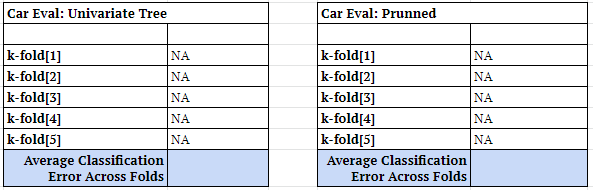
\includegraphics[scale=.7]{CarEval_Results}\newline
\end{table}

\begin{table}[h]
		\centering
		\caption{Breast Cancer: ID3 - Experimental Results}
		\label{tab:table2}
		%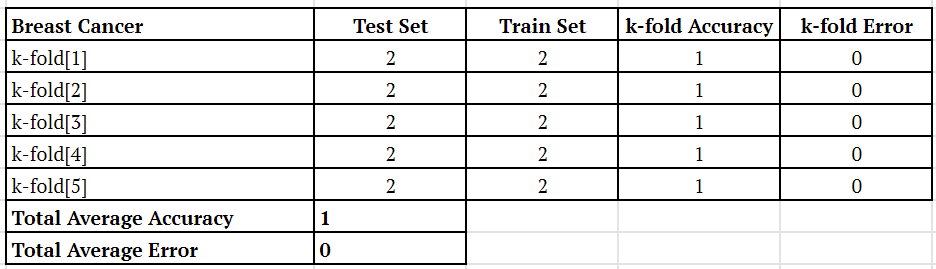
\includegraphics[scale=.7]{BC_Results}\newline
\end{table}
\newpage

\begin{table}[h]
		\centering
		\caption{Congressional Vote: ID3 - Experimental Results}
		\label{tab:table3}
		%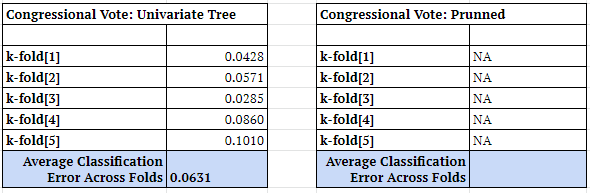
\includegraphics[scale=.7]{CongVote_Results}\newline
\end{table}

\begin{table}[h]
	\centering
	\caption{Albalone: CART - Experimental Results}
	\label{tab:table4}
	%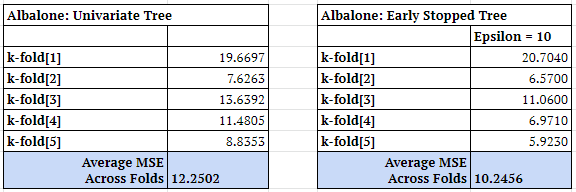
\includegraphics[scale=.7]{Albalone_Results}\newline
\end{table}

\begin{table}[h]
	\centering
	\caption{Computer Hardware: CART - Experimental Results}
	\label{tab:tale5}
	%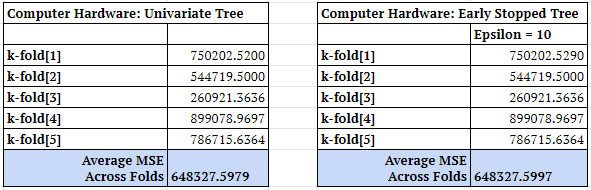
\includegraphics[scale=.7]{CompHardware_Results}\newline
\end{table}

\begin{table}[h]
	\centering
	\caption{Forest Fires: CART - Experimental Results}
	\label{tab:table6}
	%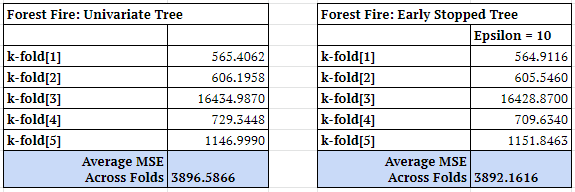
\includegraphics[scale=.7]{ForestFire_Results}\newline
\end{table}

\newpage
\newpage


\section{Discussion}
\hspace*{10mm} The hypothesis that was presented at the start of this report for the both the classification and regression tasks the trees that are error pruned or early stopped will perform better than trees that are grown uni-variate to completion.\\
\hspace*{10mm} Looking at the classification data sets, the only data set that was able to run to full completion was the Congressional Vote data set. The Car Evaluation and Breast Cancer data sets, were unable to be fully built, this was most likley due to an implementation error as they never returned from the recursive calls that were used to build the trees. Too much time was spent trying to debug these data sets, such that Prunning was also unable to be implemented in time for submission. This is unfortunate, as no meaningful comparisons can be made towards the support of the hypothesis presented in the Introduction section. However, it does afford some lessons learned that will be applied to next implementation attempts of such algorithms.  \\
\hspace*{10mm} Looking at the Regression data sets, the values of $\epsilon$ that were evaluated were 0, 0.01, 0.1, 1, 10. During the tuning process it was determined that 10 was the optimal value to use for $\epsilon$ and it was observed that there was not large difference between the results obtained for $\epsilon$ values such as 0, 0.01, 0.1, 1. One reason for this might that due to range of possible values for the prediction value in the regression data sets, a large $\epsilon$ makes a larger impact as it allows for the account of outliers in the data. The Albalone data set was the only one that had measurable improvement, with an Average MSE dropping from 12.5 to 10.2 between the uni-variate tree and the early stopped tree. The Forest Fire and Computer Hardware data sets, did not see measurable improvements between the uni-variate tree and the early stopped tree. The Albalone data set did not include multiple features that needed to be one hot encoded, Sex was the only attributes and it only provided 3 options to one hot encode. The Forest Fire and Computer Hardware data sets on the other hand had multiple attributes that were one hot encoded, and each of those attributes had multiple options that were derived because of this one hot encoding. It is possible that one hot encoding this data was the wrong approach, and alternative methods should have been used, such as dropping those attributes completely. Since one hot encoding offers only 0 or 1 for the options the splits that will be generated when performing the regression might be highly skewed towards on particular branch as the data is classified through the regression tree.\\
\section{Conclusion}
\hspace*{10mm} Overall there seemed to be some trends in the data that supported the hypothesis, that both the classification and regression tasks the trees that are error pruned or early stopped will perform better than trees that are grown uni-variate to completion. However, it was noted that implementation issues did not allow for the classification data sets to have many meaningful trees built, so no conclusions can be drawn toward the hypothesis for classification. The lesson learned that can be applied is that for recursive problems it is important to have debugging methodology in place that cane be used to determine quickly at what level of the recursion were issue encountered.\newline
\hspace*{10mm} The regression data sets were able to be fully grown and implement early stopping. It was noticed that early stopping in some cases did tend to improve the MSE that was obtained fold to fold, but there were other details such as one hot encoding that might have impacted the results for other data sets, that had more data that needed one hot encoding to be applied to.\newline
\hspace*{10mm} A suggested area of future work, after fixing basic implementation details, would be to consider other methods of prunning or early stopping. For Classification and Regression machine learning problems, other such methods include Cost-Complexity Pruning.\newline

\section{References}
1. Alpaydin, E. (2004). Introduction to machine learning (Oip). Mit Press. 

\newpage


\end{document}